

\section{Identifying high-$z$ galaxies with Euclid}

With one visible and 3 near-infrared bands \euclid\ provides the ability to robustly identify galaxies at high-redshift $z>6$ via the Lyman-$\alpha$/limit break. To demonstrate \euclid's capabilities we run a simple simulation in which we generate synthetic photometry assuming a simple $\beta$ model. In this model the underlying rest-frame ultraviolet spectrum is described by a simple power-law: $L_{\nu}\propto \lambda^{\beta+2}$ with ISM/IGM abosorption described by MADAU96.

We then add noise assuming the \euclid\ point-source depths and use the {\sc eazy} \insref\ photometric redshift code.



\begin{figure}
	\centering
	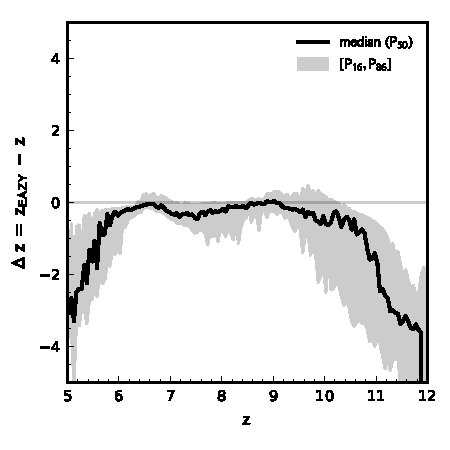
\includegraphics[width=0.45\textwidth]{./figures/beta/beta_dz.pdf}
	\caption{The difference between the median photometric redshift $z_{\rm EAZY}$ and the input redshift $z$ ($\Delta z = z_{\rm EAZY} - z$) as a function of input redshift. The solid line shows the median value of $\Delta z$ while the shaded region shows the central 68\% range. Input models assume a uniform distribution of UV continuum slopes $\beta\in[-3,0]$ and luminosities. Only galaxies with ${\rm S/N(H)}=5-20$ are included in the figure.\label{fig:beta_dz}}
\end{figure}

\begin{figure}
	\centering
	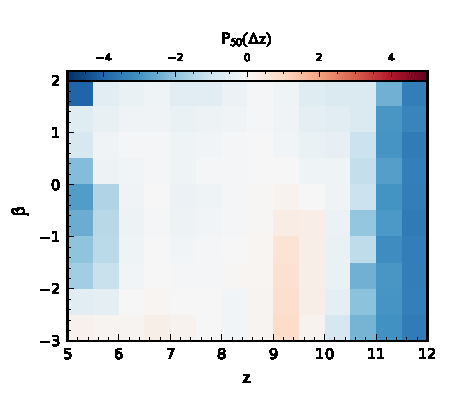
\includegraphics[width=0.45\textwidth]{./figures/beta/beta_bias.pdf}
  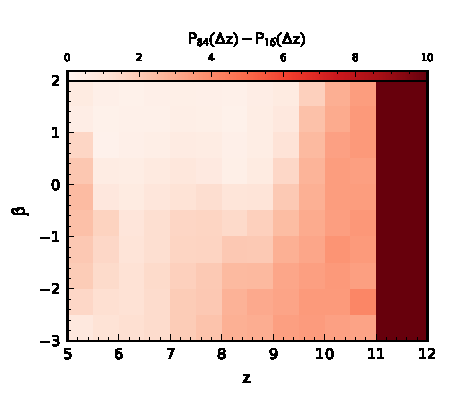
\includegraphics[width=0.45\textwidth]{./figures/beta/beta_scatter.pdf}
	\caption{The measured photometric redshift bias (top) and scatter (bottom) as a function of input redshift ($z$) and UV continuum slope ($\beta$). \label{fig:beta_bias_scatter}}
\end{figure}


\onecolumn

\begin{figure}
	\centering
	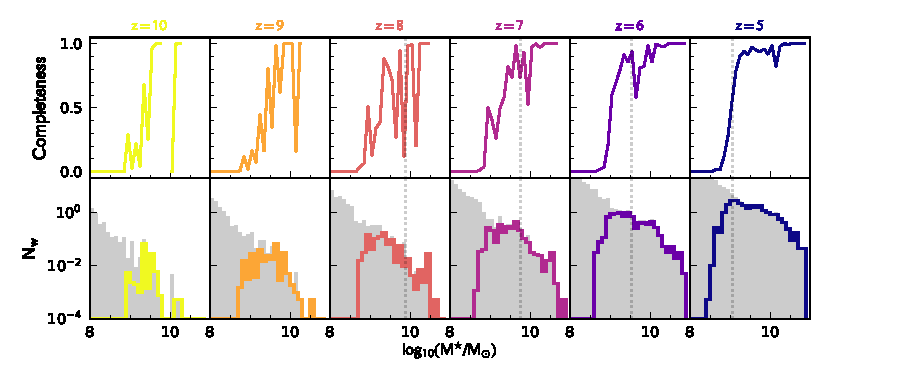
\includegraphics[width=0.9\textwidth]{figures/physical/hist_Mstar_30.pdf}
	\caption{Completeness of the stellar mass function of galaxies accessible to Euclid (top) and numbers of objects accessible to Euclid at each redshift (bottom). \textcolor{red}{*** What is the weighting here again? bottom panel seems to be more than just numbers of objects ***}}
	\label{fig:physical:mstar}
\end{figure}

\begin{figure}
	\centering
	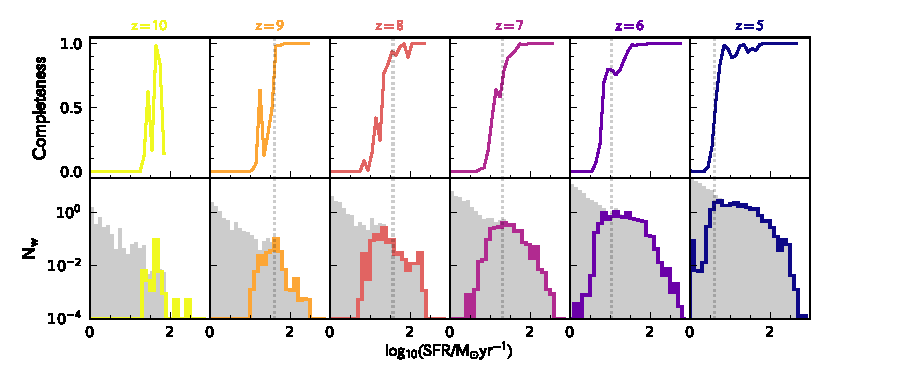
\includegraphics[width=0.9\textwidth]{figures/physical/hist_SFR_inst_30.pdf}
	\caption{Completeness of the star formation rate function of galaxies accessible to Euclid (top) and numbers of objects accessible to Euclid at each redshift (bottom). \textcolor{red}{*** What is the weighting here again? bottom panel seems to be more than just numbers of objects ***}}
	\label{fig:physical:sfr}
\end{figure}

\begin{figure}
	\centering
	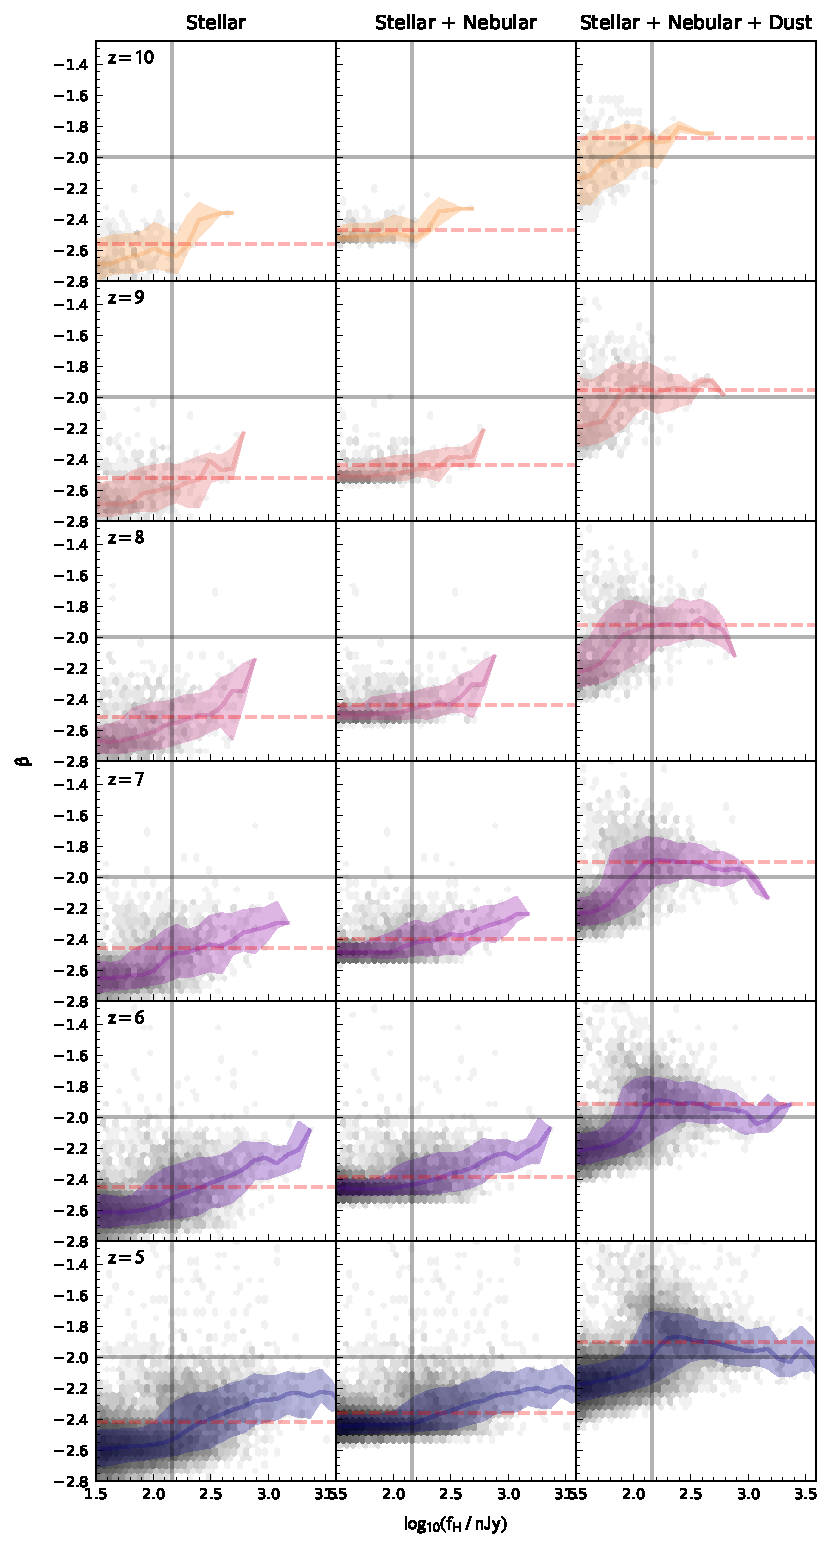
\includegraphics[width=0.65\textwidth]{./figures/beta/beta_all}
	\caption{UV continuum slope $\beta$ vs. $\rm H$-band flux for all considered EoR redshifts. The solid line shows the median of the $\rm \beta$ distribution and the shaded region shows the corresponding 84\% - 16\% range. The vertical lines show the $\rm H = 26$ limit, horizontal black line shows $\rm \beta = -2$ (to guide the eye) and the horizontal red dashed line shows median $\rm \beta$ for galaxies accessible to \euclid. \label{fig:beta_all} \textcolor{red}{*** remake plot with xlimit set so that the labels don't overlap ***}}
\end{figure}